\section{sFlow}
\subsection{sFlow}
\subsubsection{Principi}
\begin{itemize}
\item Non si pretenda di essere veloce come la rete che si vuole monitorare: si perderanno comunque dei dati.
\item Anche se si riesce a monitorare tutto, si avranno comunque delle difficolt� nel gestire tutti i flussi generati.
\item Analizzare 1 pacchetto ogni X pacchetti (campionamento).
\item Pi� pacchetti si analizza, pi� si avranno dati precisi.
\item Se la rete � troppo veloce, si aumenta il valore di campionamento.
\end{itemize}

\subsubsection{Architettura}
\begin{minipage}{.58\textwidth}
  \begin{itemize}
  \item La sonda campiona il traffico.
  \item I pacchetti campione sono spediti (nel formato sFlow) al collezionatore.
  \item Periodicamente la sonda invia le statistiche raccolte sulle interfacce (i contatori MIB II SNMP) dentro i pacchetti sFlow.\\
    I pacchetti sono usati per ``scalare'' il traffico.
  \end{itemize}
\end{minipage}
\hspace{.05\textwidth}
\begin{minipage}{.27\textwidth}
  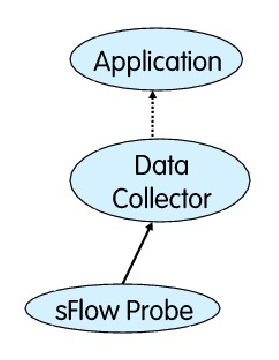
\includegraphics{figure/Architettura_sFlow.eps}
\end{minipage}

\subsubsection{Specifiche}
\begin{itemize}
\item Specificato nelle RFC 3176 (RFC informative) proposte dalla InMon Inc..
\item Definisce:
  \begin{itemize}
  \item Formato del pacchetto sFlow (UDP, no SNMP).
  \item Un MIB SNMP per accedere ai dati sFlow raccolti\\
    (\url{http://support.ipmonitor.com/mibs/SFLOW-MIB/tree.aspx}).
  \end{itemize}
\item L'architettura di sFlow � simile a quella di NetFlow: la sonda spedisce i pacchetti sFlow al collezionatore.
\item La sonda sFlow � in pratica uno sniffer che cattura 1 pacchetto su X (la proporzione di default � 1:400).
\item Questi pacchetti sono spediti al collezionatore codificati nel formato sFlow.
\item Periodicamente la sonda spedisce altri pacchetti sFlow che contengono statistiche sulle interfacce di rete (ad esempio i contatori del traffico dell'interfaccia), statistiche che sono usate per scalare i dati raccolti.
\item Usando delle formule statistiche � possibile produrre un rapporto abbastanza preciso del traffico.
\item $\%Errore\ di\ campionamento \le 196 \times \sqrt{\frac{1}{numero\ di\ campioni}}$
  \bigskip \\
  \url{http://www.sflow.org/packetSamplingBasics/}.
\item sFlow � scalabile (basta incrementare il rapporto di campionamento) anche sulle 10 GB e oltre.
\item ntop.org � parte del consorzio sFlow.org.
\end{itemize}

\subsubsection{Il pacchetto}

{\footnotesize
\begin{verbatim}
struct sample_datagram_v5 {
   address agent_address          /* IP address of sampling agent,
                                     sFlowAgentAddress. */
   unsigned int sub_agent_id;     /* Used to distinguishing between datagram
                                     streams from separate agent sub entities
                                     within an device. */
   unsigned int sequence_number;  /* Incremented with each sample datagram
                                     generated by a sub-agent within an
                                     agent. */
   unsigned int uptime;           /* Current time (in milliseconds since device
                                     last booted). Should be set as close to
                                     datagram transmission time as possible.
                                     Note: While a sub-agents should try and
                                           track the global sysUptime value
                                           a receiver of sFlow packets must
                                           not assume that values are
                                           synchronised between sub-agents. */
   sample_record samples<>;        /* An array of sample records */
}

struct flow_sample {
   unsigned int sequence_number;  /* Incremented with each flow sample
                                     generated by this source_id.
                                     Note: If the agent resets the
                                           sample_pool then it must
                                           also reset the sequence_number.*/
   sflow_data_source source_id;   /* sFlowDataSource */
   unsigned int sampling_rate;    /* sFlowPacketSamplingRate */
   unsigned int sample_pool;      /* Total number of packets that could have
                                     been sampled (i.e. packets skipped by
                                     sampling process + total number of
                                     samples) */
   unsigned int drops;            /* Number of times that the sFlow agent
                                     detected that a packet marked to be
                                     sampled was dropped due to
                                     lack of resources. The drops counter
                                     reports the total number of drops
                                     detected since the agent was last reset.
                                     A high drop rate indicates that the
                                     management agent is unable to process
                                     samples as fast as they are being
                                     generated by hardware. Increasing
                                     sampling_rate will reduce the drop
                                     rate. Note: An agent that cannot
                                     detect drops will always report
                                     zero. */

   interface input;               /* Interface packet was received on. */
   interface output;              /* Interface packet was sent on. */

   flow_record flow_records<>;    /* Information about a sampled packet */
}
\end{verbatim}
}

\begin{figure}[htbp]
  \centering
  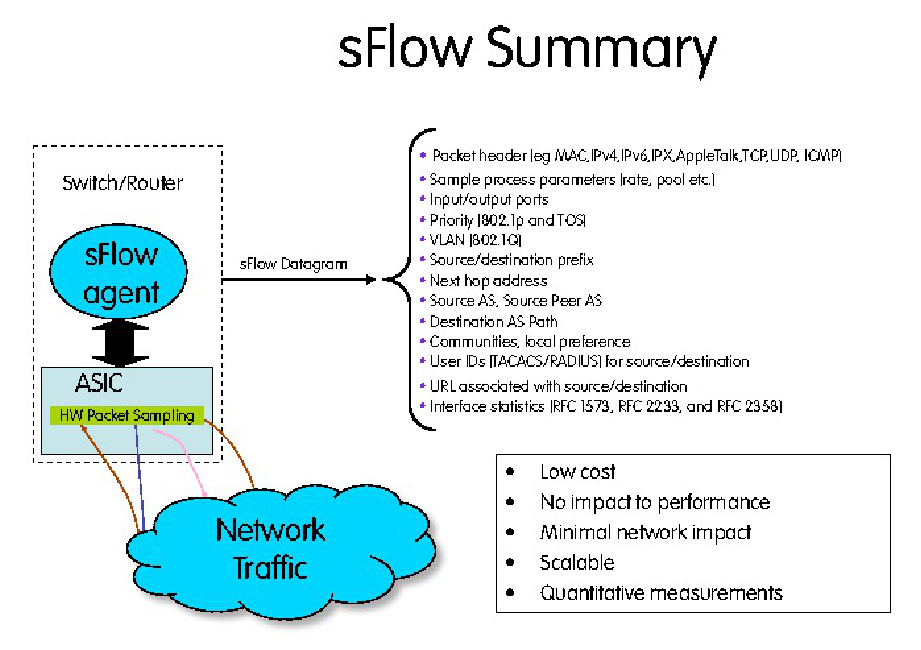
\includegraphics{figure/sFlow_sommario.eps}
  \caption{sFlow: sommario}
\end{figure}

\begin{figure}[htbp]
  \centering
  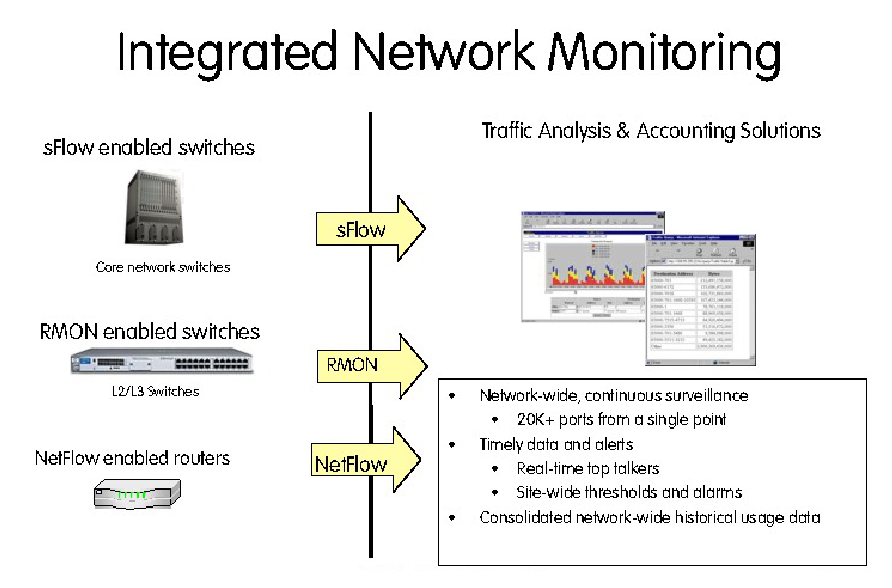
\includegraphics{figure/sFlow_monitoraggio_di_rete_integrato.eps}
  \caption{Monitoraggio di rete integrato}
\end{figure}

\subsubsection{sFlow verso NetFlow}
\begin{tabular}{|l|c|c|}
  \hline
  & sFlow & NetFlow\\
  \hline
  Ambiente nativo & Switch & Router\\
  \hline
  Velocit� a cui pu� operare & Multigigabit & 1 GB o meno\\
  \hline
  Campionamento & Sempre & Qualche volta\\
  \hline
  Monitoraggio & Statistico & Accurato (nessuna perdita)\\
  \hline
\end{tabular}

\subsection{RADIUS [RFC 2139, 1997]}
RADIUS � l'acronimo di  Remote Authentication Dial In User Service, specificato nelle seguenti RFC:
\begin{itemize}
\item Protocollo di autenticazione\\
  Rigney, C., Rubens, A., Simpson, W, and Willens, S.; Remote Authentication Dial In User Service (RADIUS), RFC 2138, January 1997.
\item Gestione dei dati\\
  Rigney, C.; RADIUS Accounting, RFC 2139, January 1997.
\end{itemize}

\subsubsection{RADIUS}
RADIUS � importante perch�:
\begin{itemize}
\item \`E il protocollo pi� usato per implementare l'autenticazione sui dispositivi di rete.
\item Usato per la fatturazione sulle reti cablate (wired lines) (ad esempio ADSL, Modem).
\item Abilita la gestione della durata della connessione o della quantit� di dati.
\item Supportato da tutti i dispositivi di rete (esclusi quelli di basso costo).
\end{itemize}

\subsubsection{Protocollo: le primitive}
La figura \ref{RADIUS} mostra un esempio di come il client RADIUS (il server per i clienti che intendono utilizzare la rete) e il server RADIUS (il server che gestisce gli account dei clienti) si scambiano i messaggi al fine di autenticare un cliente. Se il server RADIUS risponde positivamente alla richiesta di accounting, allora il cliente � libero di utilizzare la rete, altrimenti il client RADIUS gli nega l'accesso.
\bigskip

Access Request ($client \rightarrow server$):
\begin{itemize}
\item Richiesta per accedere al servizio di rete (ad esempio autenticazione dell'utente).
\item Possibile risposta:
  \begin{itemize}
  \item Access Accept ($server \rightarrow client$).
  \item Access Reject ($server \rightarrow client$).
  \item Access Challenge ($server \rightarrow client$): usata per l'autenticazione CHAP.
  \end{itemize}
\end{itemize}

Accounting Request ($client \rightarrow server$):
\begin{itemize}
\item Richiesta di scrivere i dati dell'account sul server degli account.
\item Risposte:
  \begin{itemize}
  \item Accounting Response ($server \rightarrow client$).
  \end{itemize}
\end{itemize}

\begin{figure}[htbp]
  \centering
  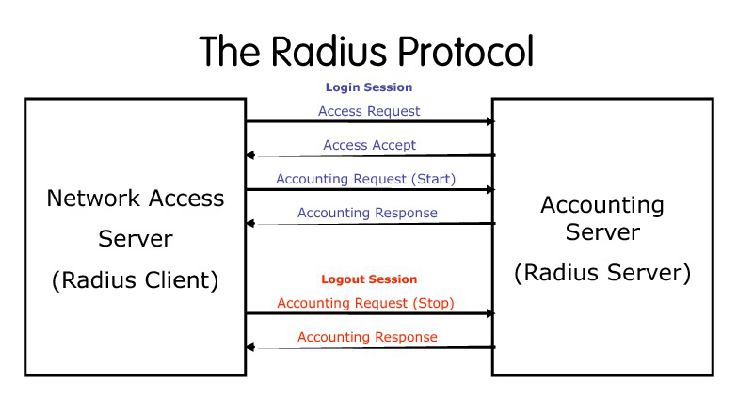
\includegraphics{figure/RADIUS_protocollo.eps}
  \caption{Il protocollo RADIUS}
  \label{RADIUS}
\end{figure}

\subsubsection{Protocollo: messaggi}
La figura \ref{RADIUS_protocollo_messaggi} mostra i messaggi scambiati dal protocollo RADIUS.
\begin{figure}[htbp]
  \centering
  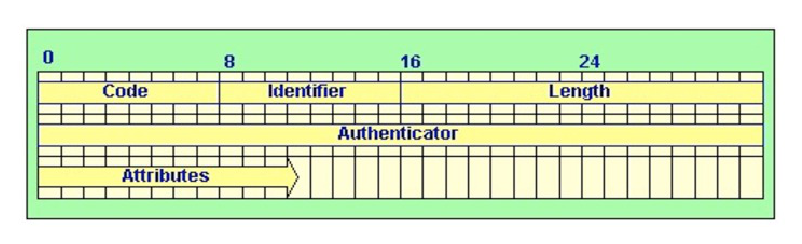
\includegraphics{figure/RADIUS_protocollo_messaggi.eps}
  \caption{Messaggi del protocollo RADIUS}
  \label{RADIUS_protocollo_messaggi}
\end{figure}
\begin{description}
\item [Code:] Il byte che contengono il comando/risposta RADIUS.
\item [Identifier:] Il byte che identifica il comando/risposta RADIUS.
\item [Length:] Lunghezza del pacchetto.
\item [Authenticator:] Valore usato per la risposta del server all'autenticazione RADIUS.
\item [Attributes:] Attributi del comando/risposta.
\end{description}

\subsection{Cattura dei pacchetti}
\subsubsection{libpcap}
Usando la libreria libpcap si fa si che tutti i pacchetti che arrivano alla scheda di rete vengano copiati e inviati al driver BPF (si veda figura  \ref{libpcap_cattura_dei_pacchetti}). Mentre il pacchetto originale segue il naturale percorso e quindi pu� anche essere scartato dalla scheda di rete se l'indirizzo MAC non corrisponde, il pacchetto copiato viene gestito dall'applicazione (quindi con l'ausilio della CPU).

\subsubsection{libpcap: esempio d'uso}

{\footnotesize
\begin{verbatim}
pcapPtr = pcap_open_live(deviceName,
     maxCaptureLen, setPromiscousMode,
     pktDelay, errorBuffer);
while(pcap_dispatch(pcapPtr, 1,
          processPacket, NULL) != -1);
void processPacket(u_char *_deviceId,
     const struct pcap_pkthdr *h,
     const u_char *p) {
     ...
}

int main(int argc, char* argv[]) {
  /* open a network interface */
descr = pcap_open_live(dev,BUFSIZ,0, 1,errbuf);
/* install a filter */
pcap_compile(descr,&fp,"dst port 80",0,netp);
pcap_setfilter(descr,&fp);
while (1) {
    /* Grab packets forever */
    packet = pcap_next(descr,&hdr);
    /* print its length */
    printf("Grabbed packet of length %d\n", hdr.len);
  }
}
\end{verbatim}
}

\begin{figure}[htbp]
  \centering
  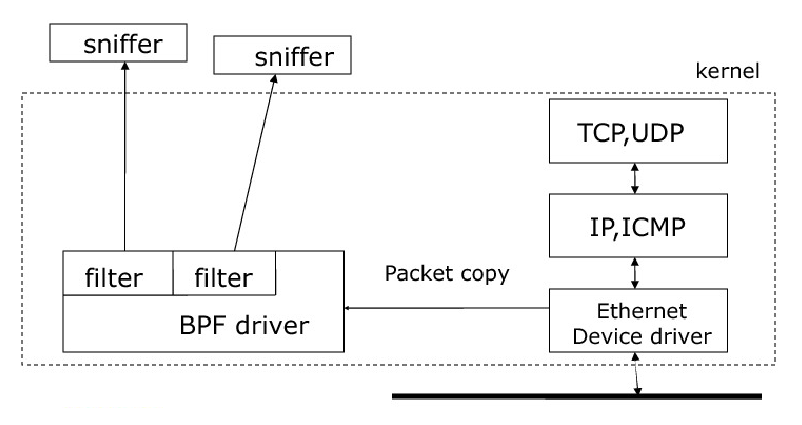
\includegraphics{figure/libpcap_cattura_pacchetti.eps}
  \caption{libpcap: cattura dei pacchetti}
  \label{libpcap_cattura_dei_pacchetti}
\end{figure}

\subsubsection{Problemi comuni con la cattura dei pacchetti}
\begin{itemize}
\item Problemi di sicurezza:
  \begin{itemize}
  \item Viene catturato tutto il traffico di rete e non solo quello destinato all'host che ``sniffa''.
  \item Se c'� una rete switchata viene catturato solo una parte del traffico (\glstext{ARP poisoning}).
  \item L'usabilit� � limitata ha chi ha i privilegi di root\\
    Nota: questo succede anche con il comando ICMP (ad esempio ping) e perci� questo comando ha il setuid abilitato.
  \end{itemize}
\item Performance:
  \begin{itemize}
  \item Lo sniffer implica anche carico di lavoro sulla CPU perch� tutti i pacchetti catturati devono essere analizzati dal programma e non solo quelli diretti verso l'host.
  \end{itemize}
\end{itemize}

\subsubsection{Cattura dei pacchetti: soluzioni}
\begin{itemize}
\item Usare una NIC (Network Interface Cart - scheda di rete) punta sulla NPU (Network Process Unit\footnote{Una Network Process Unit (NPU) � un array di una o pi� CPU specializzate per gestire le funzioni di rete. Le NPU hanno l'obiettivo di esaminare e manipolare in maniera efficiente l'header dei pacchetti.}). Ogni moderna NIC ha un limitato numero di NPU (\glstext{multicast} e ethernet). Se si possiede un driver che sfrutta al meglio la NPU allora si possono fare anche altre cose, oltre al filtraggio per MAC address.
\item Usare una scheda programmabile (ad esempio Napatech, si veda figura \ref{cattura_napatech}).
\item Eseguire il codice di gestione/amministrazione del traffico direttamente sulla NIC (ad esempio Inter IPX Family).
\item Accesso ad alta velocit� (via mmap()) per prendere i pacchetti direttamente dalla NIC via bus PCI (ad esempio Endage DAG Card, si veda figura \ref{cattura_DAG}).
\end{itemize}

\begin{figure}[htbp]
  \centering
  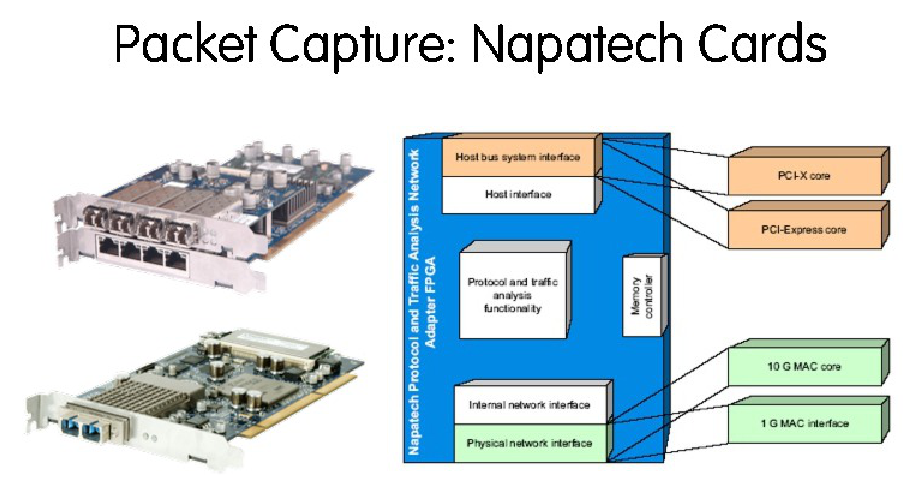
\includegraphics{figure/Network_capture_Napatech.eps}
  \caption{Cattura dei pacchetti: schede di rete Napatech}
  \label{cattura_napatech}
\end{figure}

\begin{figure}[htbp]
  \centering
  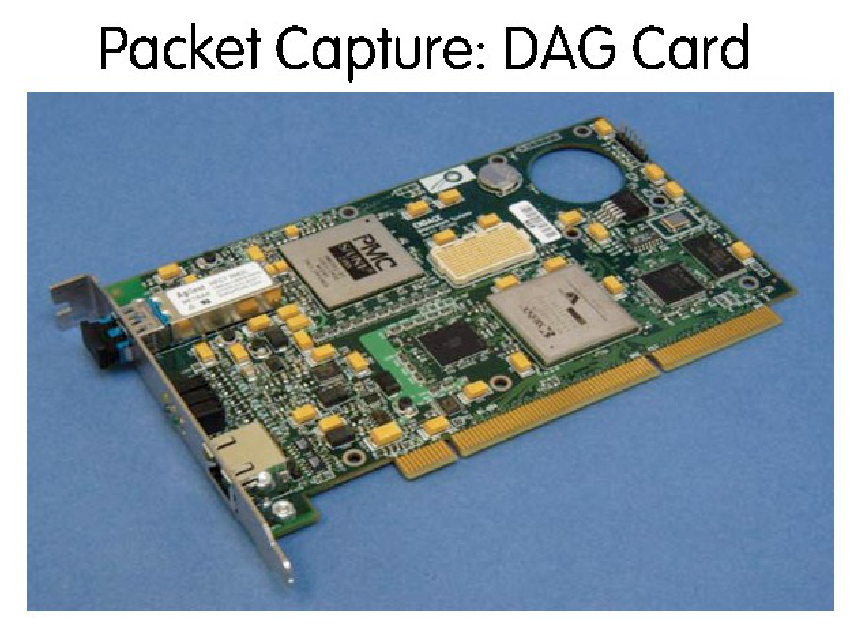
\includegraphics{figure/Network_capture_DAG.eps}
  \caption{Cattura dei pacchetti: scheda di rete DAG}
  \label{cattura_DAG}
\end{figure}

\begin{figure}[htbp]
  \centering
  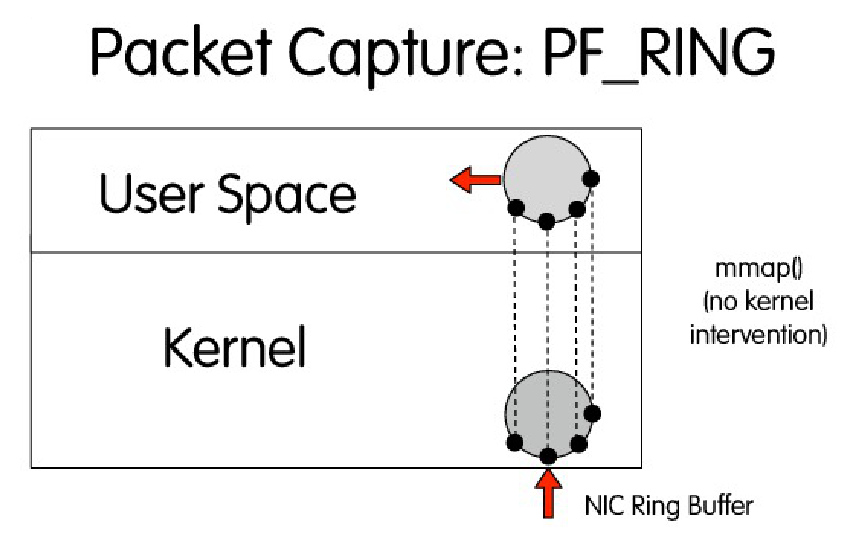
\includegraphics{figure/Network_capture_PF_Ring.eps}
  \caption{Cattura dei pacchetti: PF Ring in DNA (Direct NIC Access) mode}
\end{figure}

\subsection{Mirror del traffico: possibili soluzioni}
Hardware:
\begin{itemize}
\item Hub (ethernet in rame, token ring).
\item Divisione ottica (fibra ottica).
\item Tap (Rame/fibra) (si veda figura \ref{mirror_schede_tap})
\end{itemize}

Software:
\begin{itemize}
\item Switch Port Mirror (1:1, 1:N).
\item Switch VLAN Mirror (N:1).
\item Switch Traffic Filter/Mirroring (Juniper).
\end{itemize}

\begin{figure}[htbp]
  \centering
  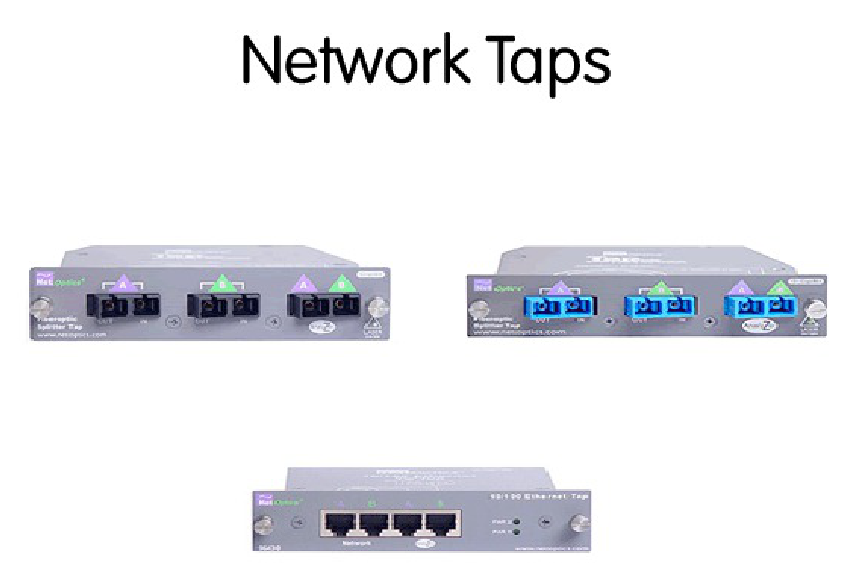
\includegraphics{figure/Network_tap.eps}
  \caption{Mirror del traffico: Tap}
  \label{mirror_schede_tap}
\end{figure}

\subsection{Collezionare i dati: RRD}
\begin{itemize}
\item RRD (\url{http://www.rrdtool.org/})
  \begin{itemize}
  \item Round Robin Database: strumento per scrivere e visualizzare i dati basato su MRTG (Multi Router Traffic Grapher).
  \item I dati sono scritti in un formato ``compresso'' che non aumenta nel tempo (i dati vengono aggregati automaticamente) lasciando inalterata la dimensione del file.
  \item Interfacce Perl/C per accedere ai dati e produrre i grafici.
  \end{itemize}
\end{itemize}

\subsubsection{Esempio in Perl}

{\footnotesize
\begin{verbatim}
$rrd = "$dataDir/$agent-$ifIndex.rrd";
if(! -e $rrd) {
    RRDs::create ($rrd, "--start",$now-1, "--step",20,
      "DS:bytesIn:COUNTER:120:0:10000000",
      "DS:bytesOut:COUNTER:120:0:10000000",
      "RRA:AVERAGE:0.5:3:288");
    $ERROR = RRDs::error;
    die "$0: unable to create `$rrd': $ERROR\n" if $ERROR;
}
    RRDs::update $rrd, "$now:$ifInOctets:$ifOutOctets";
   if ($ERROR = RRDs::error) {
    die "$0: unable to update `$rrd': $ERROR\n";
}
\end{verbatim}
}

\begin{figure}[htbp]
  \centering
  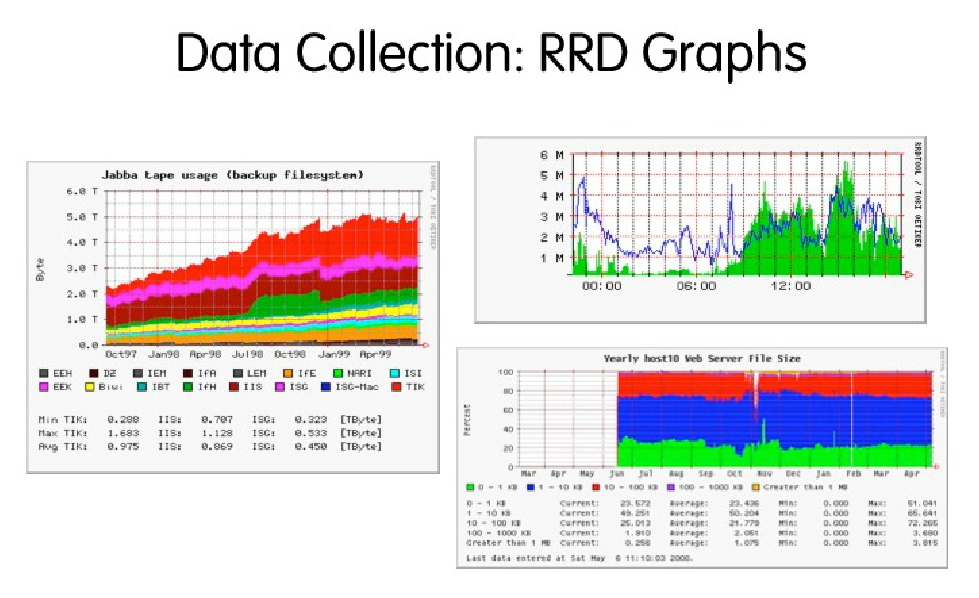
\includegraphics{figure/RRD.eps}
  \caption{Collezionare i dati: RRD}
\end{figure}

% LocalWords:  sFlow collezionatore MIB SNMP RFC InMon Inc UDP NetFlow sniffer
% LocalWords:  GB ntop org Switch Router Multigigabit RADIUS Authentication and
% LocalWords:  Dial Service Rigney Rubens Simpson Willens January Accounting PF
% LocalWords:  wired lines client accounting Access Request Accept Reject CHAP
% LocalWords:  Challenge Response Identifier Length Authenticator Attributes
% LocalWords:  libpcap BPF MAC all'host sniffa' switchata ARP poisoing ICMP NIC
% LocalWords:  setuid l'host Interface Cart NPU Process Unit array l'header IPX
% LocalWords:  multicast ethernet Napatech Family mmap Endage DAG Mirror Hub
% LocalWords:  token Port VLAN Traffic Filter Mirroring Juniper RRD Robin MRTG
% LocalWords:  Grapher Perl
